\documentclass[12pt, aspectratio=169]{beamer} % aspectratio = 43 of 169
\usepackage{color}
\usepackage{tikz}
\usepackage{transparent}

% kleuren (theme=...): red (standaard), blue, cyan, orange, green
% official=false: een mooie, maar niet-officiele stijl
% official=true: de stijl die ze ook in PowerPoint hebben, met dat blauwe blokje onderaan
% MERK OP: bij official=true is de nummering van de slides verkeerd!
\usetheme[department=winuk,official=false,theme=cyan,innovation=false,titlebgimage=imgs/screenshot-titleframe.png]{tue2008}

\mode<presentation>

\setbeamercolor{alerted text}{fg=tueblue}

% \graphicspath{{./imgs/}}

% http://stackoverflow.com/a/5971923/962603
\newenvironment{animationframe}
  {\begin{frame}}
  {\end{frame} \addtocounter{framenumber}{-1}}

\title{Building a conveyor belt editor and simulator}
\author{Thom Castermans and Willem Sonke}

\begin{document}

\begin{titleframe}
\end{titleframe}

\begin{frame}
  \frametitle{Project idea}
  \begin{columns}[c]
    \column{.6\textwidth}
      \begin{itemize}
        \item Building a conveyor belt system
        \item Simulating luggage movement
      \end{itemize}
    \column{.4\textwidth}
      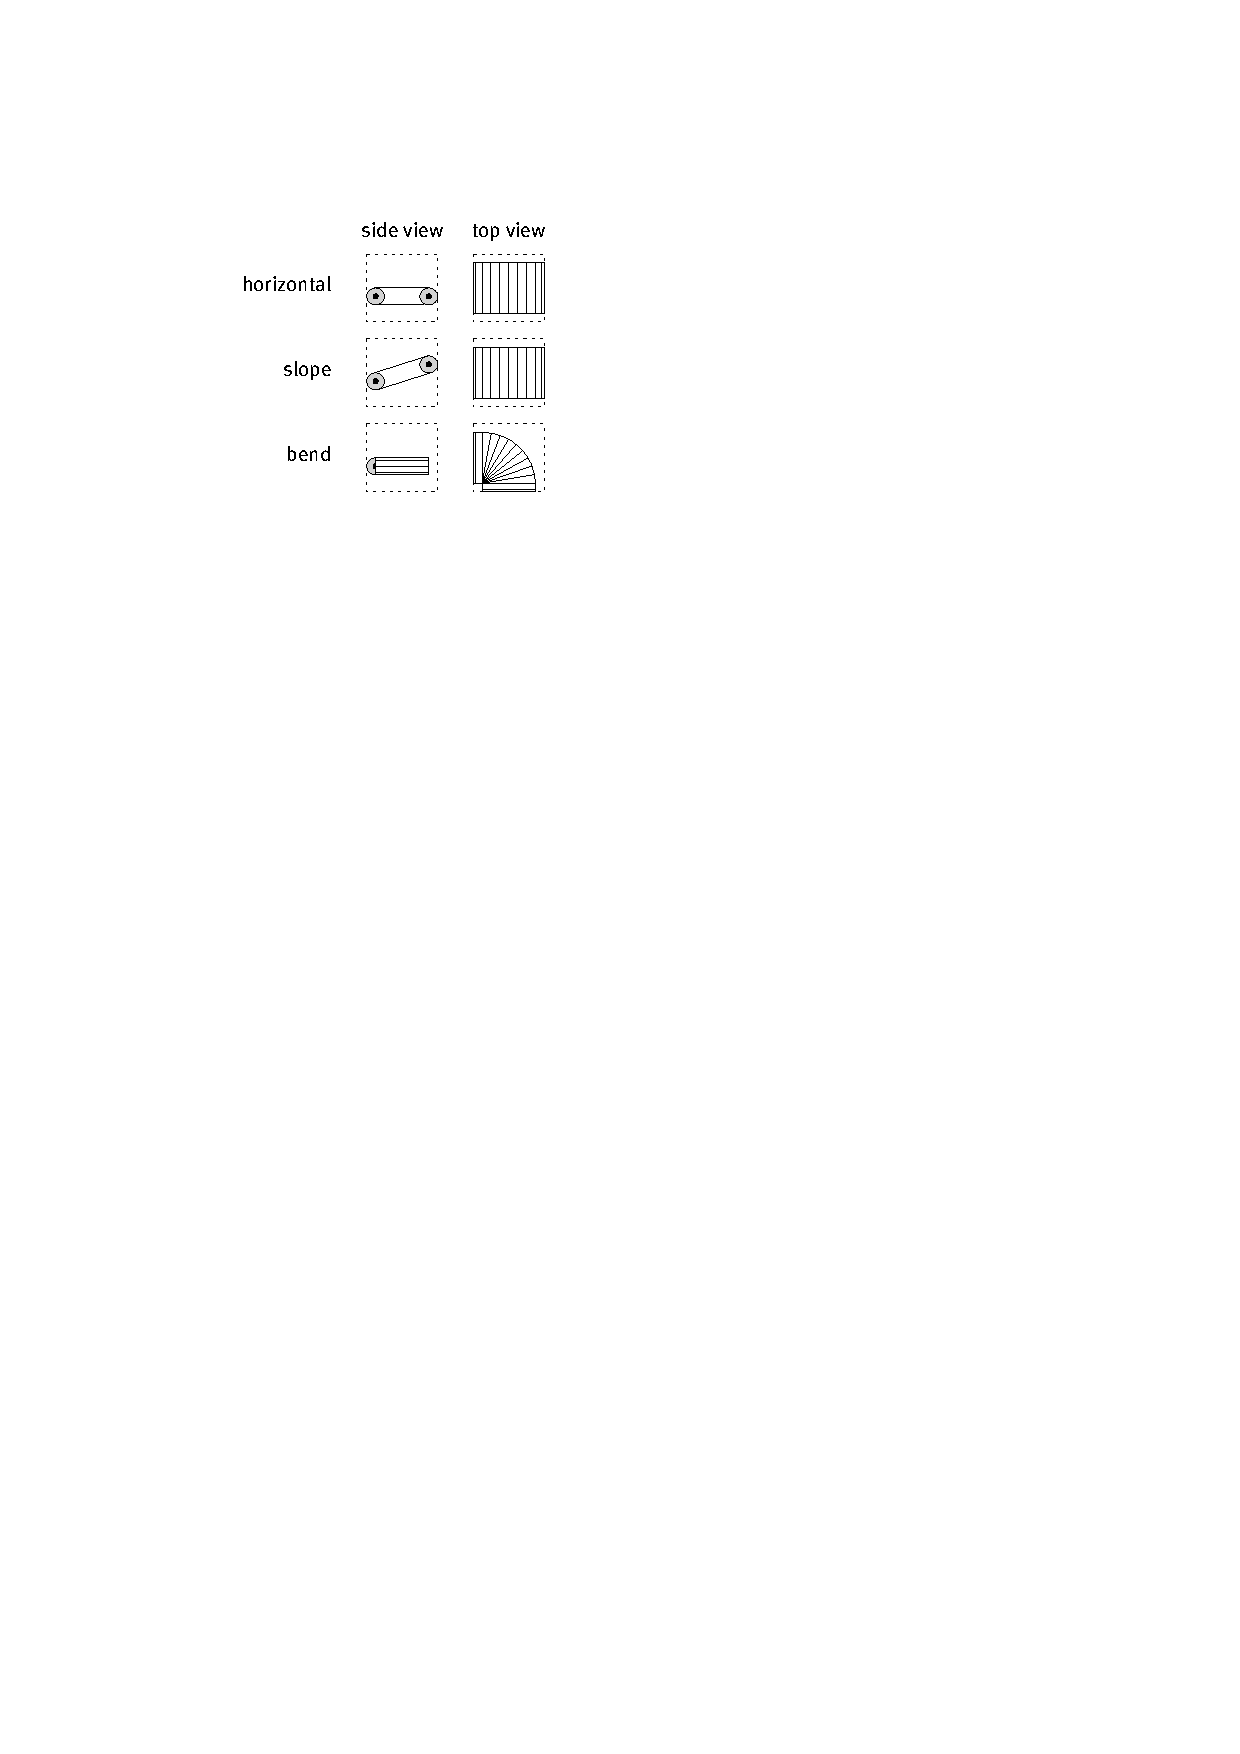
\includegraphics{imgs/sketch-blocks}
  \end{columns}
\end{frame}

% \begin{frame}
%   \frametitle{Problems\,/\,solutions}
%   \begin{itemize}
%     \item Drawing\,/\,texturizing the conveyor belts
%     \begin{itemize}
%       \item want to texturize without deformation
%       \item however, different shapes of conveyor belts
%     \end{itemize}
%   \end{itemize}
%   \begin{center}
%     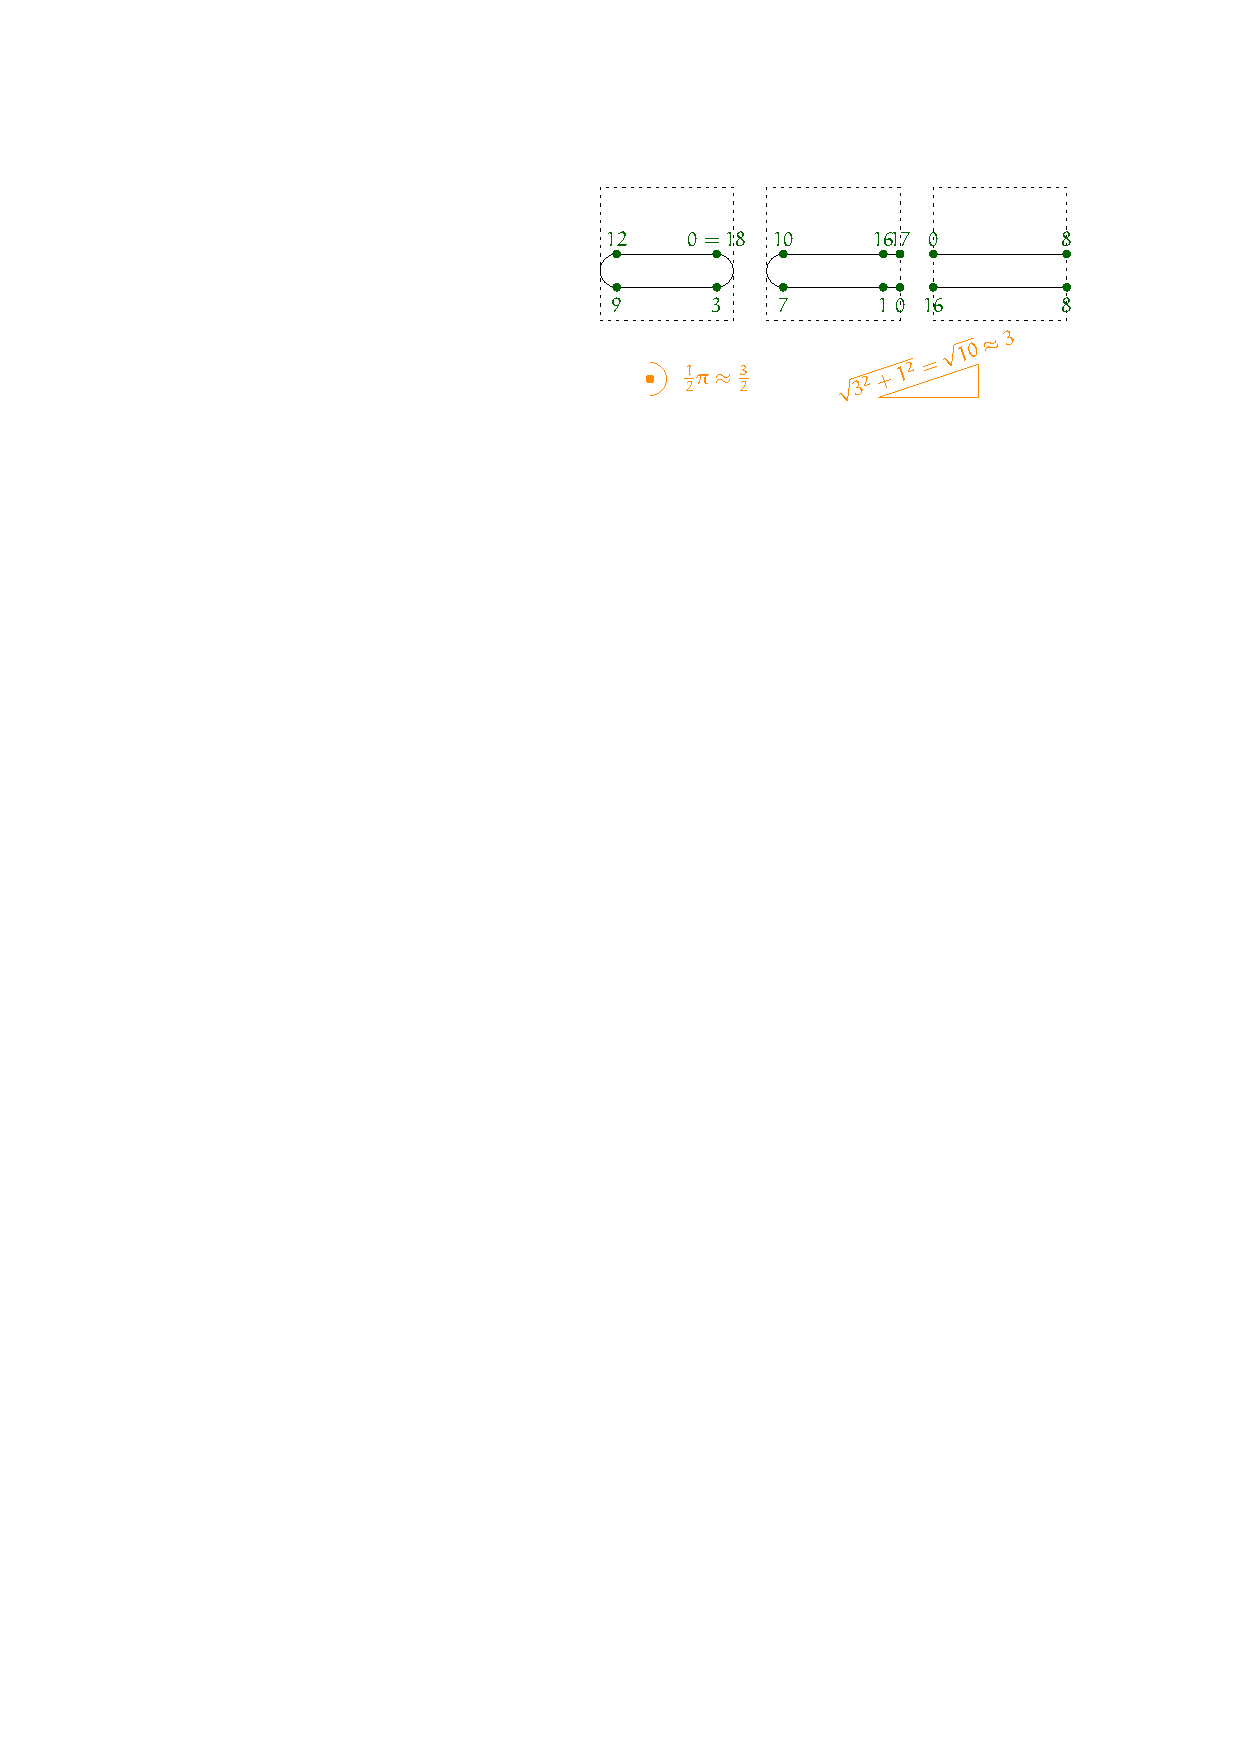
\includegraphics{imgs/sketch-texturing} % TODO [ws] graphics path doesn't seem to work? Hardcoded imgs for now
%   \end{center}
% \end{frame}

\begin{frame}
  \frametitle{New functionality since last time}
  \begin{columns}[c]
    \column{.67\textwidth}
      \begin{itemize}
        \uncover<1->{
        \item Drawing adjacent conveyor belts connected
        }
        \uncover<2->{
        \item Improving simulation
        \begin{itemize}
          \item JBullet
        \end{itemize}
        }
        \uncover<3->{
        \item Editing
        \begin{itemize}
          \item no deleting yet\ldots
        \end{itemize}
        }
        \uncover<4->{
        \item Better rendering
        \begin{itemize}
          \item shadows
        \end{itemize}
        }
        \uncover<5->{
        \item Animations in the GUI
        }
      \end{itemize}
    \column{.33\textwidth}
      \only<1>{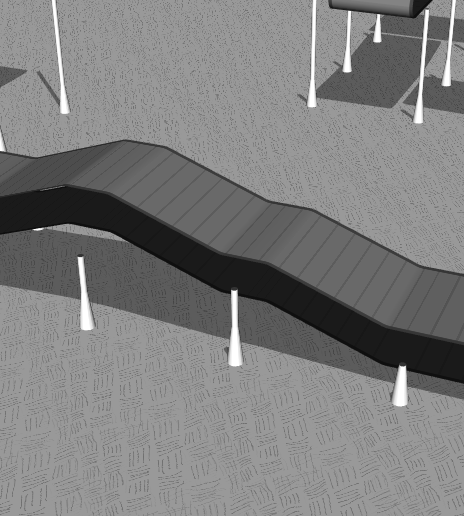
\includegraphics[height=\textwidth]{imgs/screenshot-together.png}}%
      \only<2>{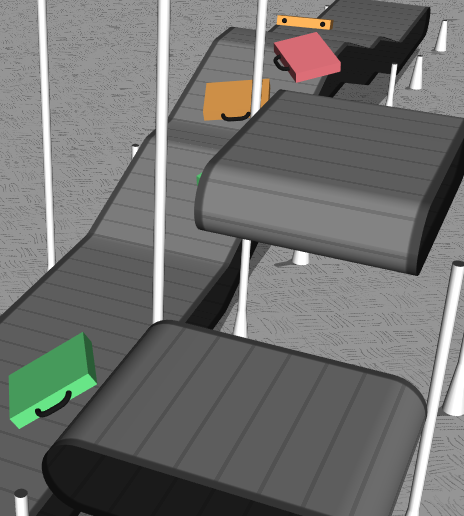
\includegraphics[height=\textwidth]{imgs/screenshot-physics.png}}%
      \only<3>{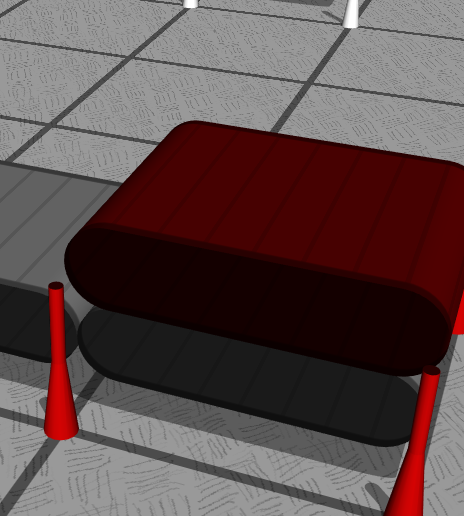
\includegraphics[height=\textwidth]{imgs/screenshot-building.png}}%
      \only<4>{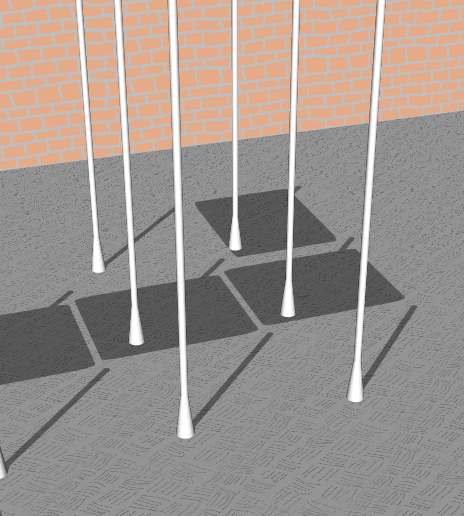
\includegraphics[height=\textwidth]{imgs/screenshot-shadows.png}}%
      \only<5>{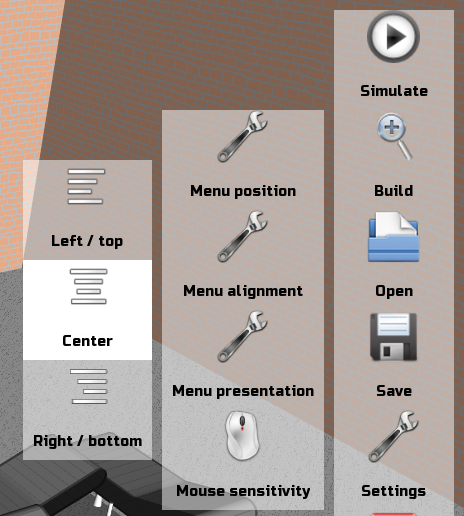
\includegraphics[height=\textwidth]{imgs/screenshot-gui.png}}%
  \end{columns}
\end{frame}

\begin{frame}
  \frametitle{Bresenham's algorithm}
  \begin{itemize}
    \item When editing, detect which block is hovered.
    \item Fast, since must potentially be done every frame.
  \end{itemize}
  \begin{center}
    % generate animation frames using a for-each loop
    \foreach \id in {1,...,11} {%
      \only<\id>{\includegraphics[scale=1]{imgs/bresenham-\id}}%
    }
  \end{center}
\end{frame}

\begin{frame}
  \frametitle{Planned work}
  \begin{columns}[c]
    \column{.67\textwidth}
      \begin{itemize}
        \uncover<1->{
        \item Deleting blocks
        }
        \uncover<2->{
        \item Adding scanners
        }
        \uncover<3->{
        \item Game-like experience, with levels
        }
        \uncover<4->{
        \item ``Sandbox mode''
        }
      \end{itemize}
    \column{.33\textwidth}
      %\uncover<1>{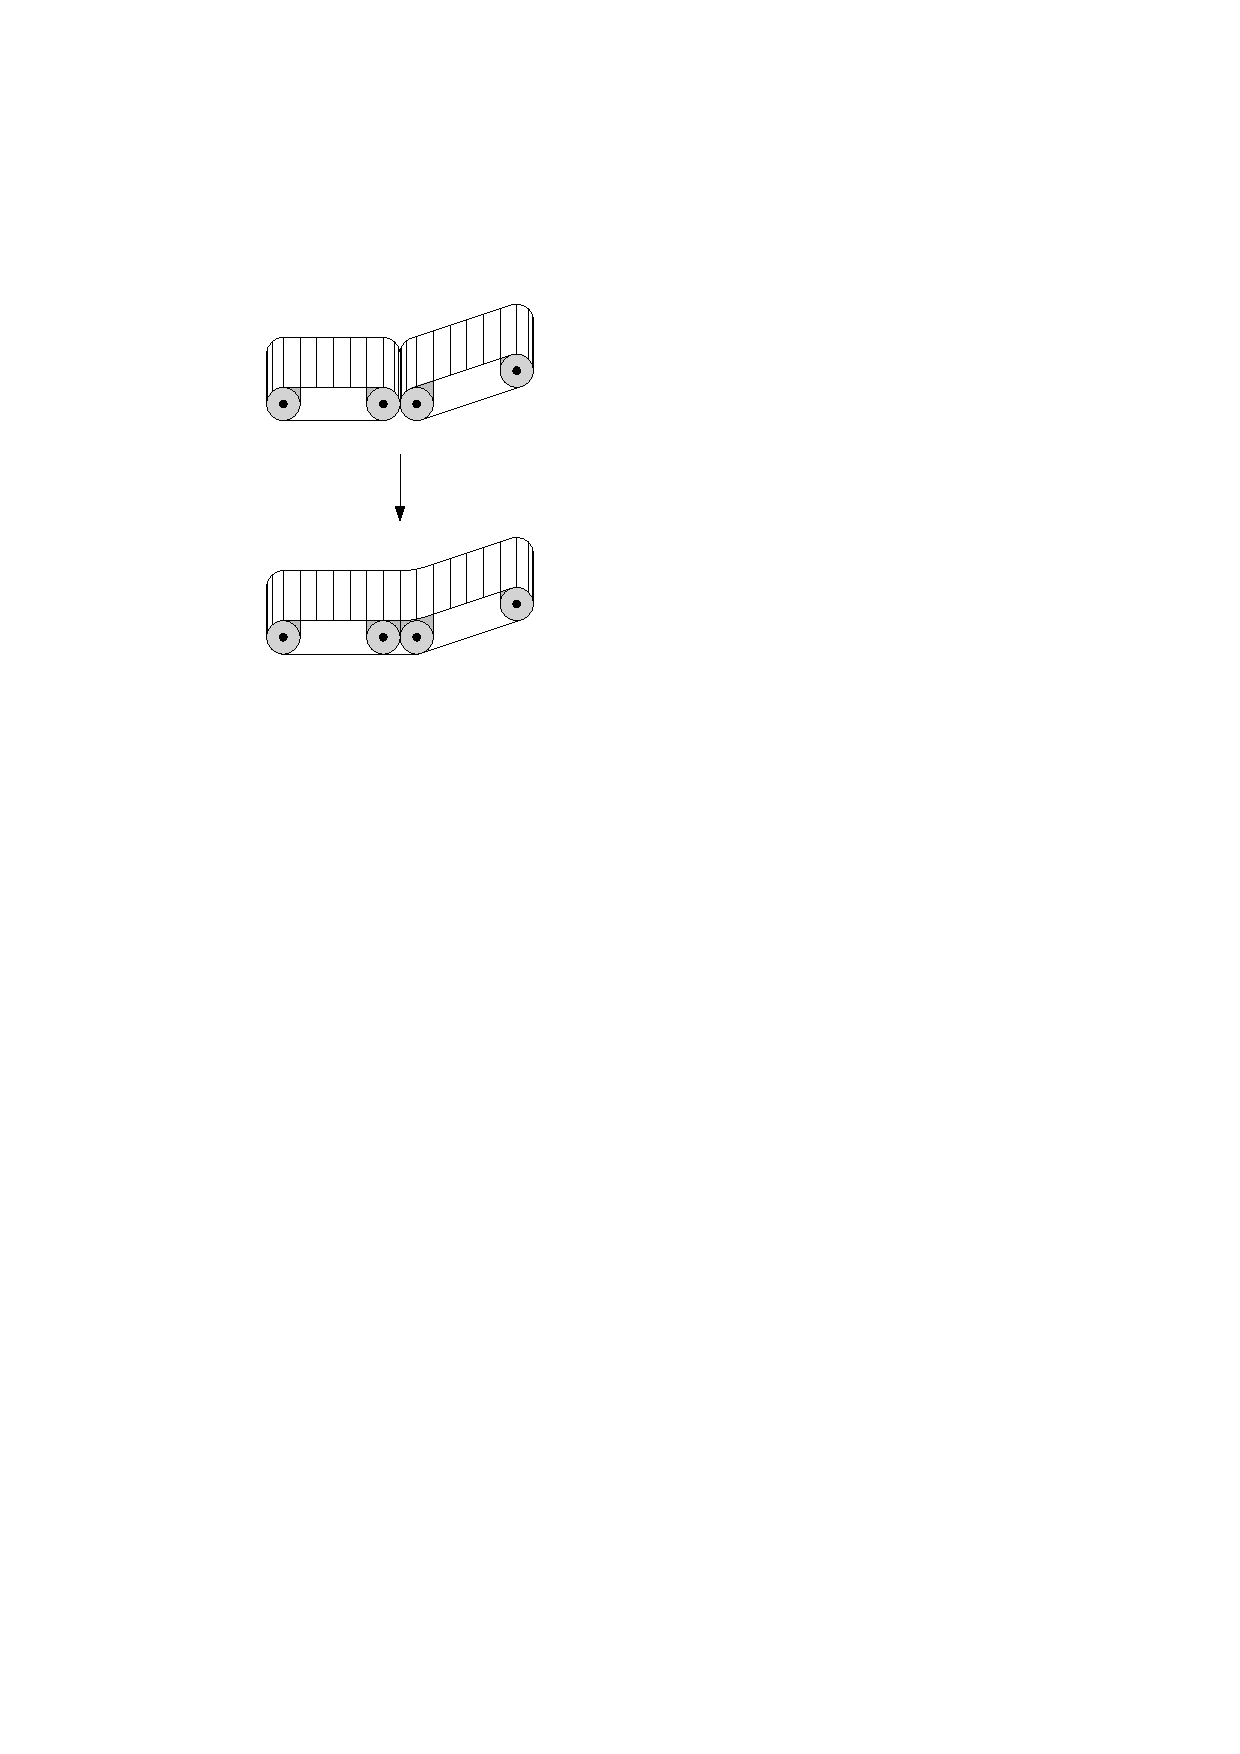
\includegraphics{imgs/sketch-adjacent-blocks}}
  \end{columns}
\end{frame}

% this does not use the graphicspath... weird
\usebackgroundtemplate{
\includegraphics[width=\paperwidth,height=\paperheight]{imgs/demo-background-011.jpg}}
\begin{frame}
  \transduration{0.25}
  \transparent{1.0}
  \begin{center}\huge\alert{Demo time!}\end{center}
\end{frame}

\end{document}
